
	Une dernière méthode de cette classe s'instituant gRepair a été proposée dans \citep{maneth2018grammar}. Ce nouveau algorithme de compression détecte de manière récursive des sous-structures répétées et les représente via des règles de grammaire.  Des requêtes spécifiques telles que l'accessibilité entre deux nœuds ou des requêtes de chemin normal peuvent ainsi être évaluées en temps linéaire (ou en temps quadratique, respectivement), sur la grammaire, permettant ainsi des accélérations proportionnelles au taux de compression. La figure \ref{gRepair} présente le résultat de cette méthode sur un exemple. 
	
	\begin{figure}[h]
			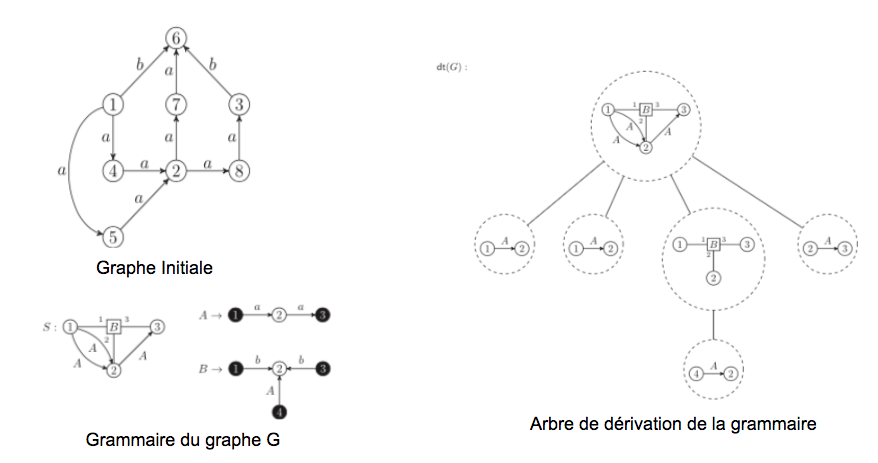
\includegraphics[scale=0.5,center]{./ressources/image/grepair.png}
			\caption[Exemple d'exécution de gRepair sur G.]{Exemple d'exécution de gRepair sur G.}
			\label{gRepair}
	\end{figure}